% Compilation : pdflatex B4.tex (deux fois).
% Document autonome : texte, formules et figures TikZ modifiables.
% Les repères « Manuscrit » renvoient aux pages du manuscrit.
\documentclass[11pt,a4paper]{article}
\usepackage[utf8]{inputenc}
\usepackage[T1]{fontenc}
\usepackage[provide=*,french]{babel}
\usepackage[scaled=.95]{helvet}
\renewcommand{\familydefault}{\sfdefault}
\usepackage{amsmath,amssymb,esint,array,tabularx}
\usepackage{geometry}
\geometry{left=15mm,right=15mm,top=18mm,bottom=18mm,headheight=14pt,headsep=6mm}
\usepackage{fancyhdr,lastpage,tikz}
\usetikzlibrary{arrows.meta,calc,decorations.pathreplacing,decorations.pathmorphing,decorations.markings,patterns,babel}
\usepackage[most]{tcolorbox}
\usepackage{enumitem,titlesec,needspace,hyperref}
\hypersetup{hidelinks,pdftitle={Dipôle électrostatique},pdfsubject={Cours de physique}}
\pagestyle{fancy}\fancyhf{}
\fancyhead[L]{\footnotesize Physique B4 - Dipôle électrostatique - inspiré par les cours de Mme Mesnil}
\fancyhead[R]{\small\thepage/\pageref{LastPage}}
\fancyfoot[R]{\small PC-PC*}
\renewcommand{\headrulewidth}{0pt}
\clubpenalty=10000\widowpenalty=10000\displaywidowpenalty=10000
\setlength{\parindent}{0pt}\setlength{\parskip}{4pt}
\setlength{\abovedisplayskip}{6pt}\setlength{\belowdisplayskip}{6pt}
\AtBeginEnvironment{center}{\setlength{\topsep}{4pt}\setlength{\partopsep}{0pt}}
\setlist[itemize]{leftmargin=5mm,itemsep=3pt,topsep=3pt,label=\(\rightarrow\)}
\setlist[enumerate]{leftmargin=6mm,itemsep=3pt,topsep=3pt}
\renewcommand{\thesection}{\Roman{section}}
\renewcommand{\thesubsection}{\thesection.\arabic{subsection}}
\titleformat{\section}{\Large\bfseries}{\thesection.}{.4em}{}
\titleformat{\subsection}{\large\bfseries}{\thesubsection.}{.4em}{}[\titlerule]
\titleformat{\subsubsection}{\normalsize\bfseries}{\alph{subsubsection})}{.5em}{}
\titlespacing*{\section}{0pt}{11pt}{6pt}
\titlespacing*{\subsection}{0pt}{9pt}{5pt}
\titlespacing*{\subsubsection}{0pt}{8pt}{4pt}
\newtcolorbox{cadre}[1][]{enhanced,sharp corners,colback=white,colframe=black,boxrule=1.1pt,left=7pt,right=7pt,top=5pt,bottom=5pt,before skip=7pt,after skip=7pt,#1}
\newif\ifinexample
\newtcolorbox{exemple}[1][]{enhanced,breakable,before upper={\inexampletrue},lines before break=3,sharp corners,colback=white,colframe=black,boxrule=.7pt,left=8pt,right=8pt,top=6pt,bottom=6pt,before skip=8pt,after skip=8pt,#1}
\tcbset{etoiles/.style={width=\dimexpr\linewidth-22mm\relax,overlay={\node[anchor=west,inner sep=0pt,font=\small] at ([xshift=2mm]frame.east) {\(#1\)};}}}
\newcommand{\zone}[1]{\tikz[baseline=(z.base)]\node[draw,circle,inner sep=1pt,font=\scriptsize,minimum size=3.5mm](z){#1};}
\newcommand{\dd}{\mathrm d}
\newcommand{\vv}{\vec v}
\newcommand{\grad}{\overrightarrow{\mathrm{grad}}}
\newcommand{\pd}[2]{\frac{\partial #1}{\partial #2}}
\newcommand{\ux}{\vec u_x}\newcommand{\uy}{\vec u_y}\newcommand{\uz}{\vec u_z}
\newcommand{\cste}{\mathrm{cste}}
\newcommand{\titr}[1]{\par\ifinexample\else\Needspace{4\baselineskip}\fi\textbf{\underline{#1}}\par\nopagebreak[3]}
\newcommand{\planpart}[2]{\par\vspace{5pt}{\bfseries #1. #2}\par}
\newcommand{\plansub}[2]{\hspace*{7mm}{\itshape #1) #2}\par}
\newcommand{\plansubsub}[1]{\hspace*{15mm}{\itshape #1}\par}
\tikzset{>=Stealth,every node/.style={font=\small},flow/.style={thick,->},edge/.style={thick}}
\newcommand{\stars}[1]{\mathord{\star}\ifnum#1>1\mkern5mu\mathord{\star}\fi\ifnum#1>2\mkern5mu\mathord{\star}\fi\ifnum#1>3\mkern5mu\mathord{\star}\fi\ifnum#1>4\mkern5mu\mathord{\star}\fi\ifnum#1>5\mkern5mu\mathord{\star}\fi}
\newenvironment{result}[1][4]{\begin{cadre}[etoiles={\stars{#1}}]}{\end{cadre}}
\newcommand{\vj}{\vec j}\newcommand{\vE}{\vec E}\newcommand{\vB}{\vec B}
\newcommand{\vPi}{\vec\Pi}\newcommand{\rot}{\overrightarrow{\mathrm{rot}}}
\newcommand{\divg}{\operatorname{div}}\newcommand{\sy}{\operatorname{sym}}
\newcommand{\D}{\mathcal D}\newcommand{\R}{\mathcal R}
\newcommand{\fig}[1]{\begin{center}#1\end{center}}
\definecolor{charge}{RGB}{155,50,165}
\definecolor{current}{RGB}{195,40,45}
\tikzset{arr/.style={thick,->},cur/.style={current,thick,->},el/.style={charge,thick,->},mag/.style={green!50!black,thick,->},pt/.style={circle,fill,inner sep=1.2pt},plane/.style={blue!55!black,thin}}
\tikzset{arr/.style={thick,->},cur/.style={red!75!black,thick,->},el/.style={purple,thick,->},pt/.style={circle,fill,inner sep=1.1pt},plane/.style={blue!60!black,thin},field/.style={red!75!black,thick,postaction={decorate},decoration={markings,mark=at position .6 with {\arrow{Stealth}}}}}
\newcommand{\ur}{\vec u_r}\newcommand{\ut}{\vec u_\theta}\newcommand{\uphi}{\vec u_\varphi}
\newcommand{\eps}{\varepsilon_0}\newcommand{\E}{\vec E}\newcommand{\dS}{\dd\vec S}\newcommand{\dM}{\dd\vec M}
\newcommand{\examtitle}[1]{\textbf{#1}\par\nobreak}

% Notation et styles des dessins. Les figures qui suivent sont intégralement vectorielles.
\newcommand{\mom}{\vec p}
\newcommand{\EE}{\vec E_{\mathrm{ext}}}
\newcommand{\EEsc}{E_{\mathrm{ext}}}
\newcommand{\VE}{V_{\mathrm{ext}}}
\newcommand{\FR}{\vec F_{\text{rés}}}
\newcommand{\MR}{\vec M_O^{\,\text{rés}}}
\newcommand{\fle}[1]{\overrightarrow{#1}}
\newcommand{\trois}[3]{\left|\begin{matrix}#1\\#2\\#3\end{matrix}\right.}
\newcommand{\remaq}{\par\textbf{Remarque :} }
\newcommand{\surdeux}[3]{\par\noindent
  \begin{minipage}[c]{#1\linewidth}\centering #2\end{minipage}\hfill
  \begin{minipage}[c]{\dimexpr\linewidth-#1\linewidth-5mm\relax}#3\end{minipage}\par}
\newcommand{\veczero}{\vec 0}
\newcommand{\bmath}[1]{\begin{cadre}\[#1\]\end{cadre}}
\newcommand{\betoile}[2]{\begin{result}[#1]\[#2\]\end{result}}
\definecolor{rougechamp}{RGB}{167,38,47}
\definecolor{violetdip}{RGB}{130,51,147}
\definecolor{vertequi}{RGB}{32,119,70}
\definecolor{bleutrait}{RGB}{43,78,149}
\tikzset{fl/.style={-{Stealth[length=2mm,width=1.5mm]},semithick},
  echamp/.style={fl,rougechamp},moment/.style={fl,violetdip},vvert/.style={fl,vertequi},
  petit/.style={font=\scriptsize,inner sep=1.4pt}, atome/.style={font=\small,inner sep=1.3pt},
  sens/.style={postaction={decorate},decoration={markings,mark=at position #1 with {\arrow{Stealth[length=1.7mm,width=1.25mm]}}}},
  sens/.default=.5}
\newcommand{\croix}[3][black]{\draw[#1,semithick] (#2,#3) ++(-.055,-.055)--++(.11,.11)
  (#2,#3) ++(-.055,.055)--++(.11,-.11);}
\newcommand{\planP}[2]{\planpart{#1}{\nameref{#2}}}
\newcommand{\planS}[2]{\plansub{#1}{\nameref{#2}}}
\newcommand{\planSS}[2]{\plansubsub{#1) \nameref{#2}}}
\newcommand{\eau}[2]{% molécule d'eau : l'axe local x est orienté de O vers les H
  \begin{scope}[shift={#1},rotate=#2]
  \draw[thin](.10,.075)--(.44,.34) (.10,-.075)--(.44,-.34);
  \draw[thin](-.18,.02)--(-.11,.15) (-.18,-.02)--(-.11,-.15);
  \node[atome,font=\scriptsize] at(0,0){O};
  \node[atome,font=\scriptsize] at(.56,.42){H};\node[atome,font=\scriptsize] at(.56,-.42){H};
  \end{scope}}
\newcommand{\equilibrefig}[1]{\begin{tikzpicture}
  \draw[fl](-1.25,0)--(1.42,0) node[right]{$\EE$};
  \draw[moment] (#1: -1.0)--(#1:1.12) node[above]{$\mom$};
  \draw[violetdip,thin,->] (#1:.56) arc[start angle=#1,end angle=6,radius=.56];
  \draw[violetdip,semithick,fill=white](0,0)circle(.105);
  \draw[violetdip,thin](-.073,-.073)--(.073,.073)(-.073,.073)--(.073,-.073);
  \node[petit,violetdip,below]at(.12,-.26){$\vec M_O$};
  \end{tikzpicture}}
\begin{document}
{\raggedright\fontsize{27}{31}\selectfont\bfseries Dipôle électrostatique\par}
\planP{I}{sec:intro}
\planS{1}{sec:def}
\planS{2}{sec:nature}
\planSS{a}{sec:molecules}
\planSS{b}{sec:induit}
\planP{II}{sec:creation}
\planS{1}{sec:sym}
\planS{2}{sec:pot}
\planS{3}{sec:champ}
\planS{4}{sec:carte}
\planP{III}{sec:actions}
\planS{1}{sec:uniforme}
\planS{2}{sec:variable}
\planS{3}{sec:energie}
\planP{IV}{sec:applications}
\planS{1}{sec:multi}
\planS{2}{sec:pol}
\planS{3}{sec:solv}
\planS{4}{sec:vdw}
\vspace{3mm}

% Manuscrit, pages 1 et 2.
\section{Introduction}\label{sec:intro}
\subsection{Définition}\label{sec:def}
\begin{cadre}
Un dipôle est un ensemble de deux charges ponctuelles opposées, \(+q\) et \(-q\)
(\(q>0\)), situées en deux points distincts, respectivement \(P\) et \(N\).
\fig{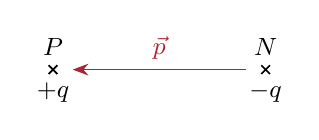
\begin{tikzpicture}
\croix{0}{0}\croix{2.7}{0}
\node[above]at(0,.06){$P$};\node[below]at(0,-.04){$+q$};
\node[above]at(2.7,.06){$N$};\node[below]at(2.7,-.04){$-q$};
\draw[echamp](2.45,0)--(.25,0)node[midway,above]{$\mom$};
\end{tikzpicture}}
\end{cadre}
\begin{cadre}\textbf{Moment dipolaire}
\[\mom=q\,\fle{NP}.\]
Unité : \(\mathrm{C\,m}\).
\end{cadre}
\remaq l'unité \(\mathrm{C\,m}\) n'est pas adaptée à l'échelle des molécules :
pour une charge de l'ordre de \(10^{-19}~\mathrm C\) et une distance de l'ordre de
\(1~\text{\AA}\), le moment est de l'ordre de \(10^{-29}~\mathrm{C\,m}\).
On introduit le debye : \(1~\mathrm D=1{,}33\times10^{-29}~\mathrm{C\,m}\).\label{err:debye}

\remaq un \textbf{dipôle rigide} est insensible aux conditions extérieures :
la charge \(q\) et la distance \(NP\) restent constantes.

% Manuscrit, pages 2 à 5.
\subsection{Les dipôles dans la nature}\label{sec:nature}
\subsubsection{Molécules polaires}\label{sec:molecules}
\begin{exemple}
Cf. cours de chimie.
\fig{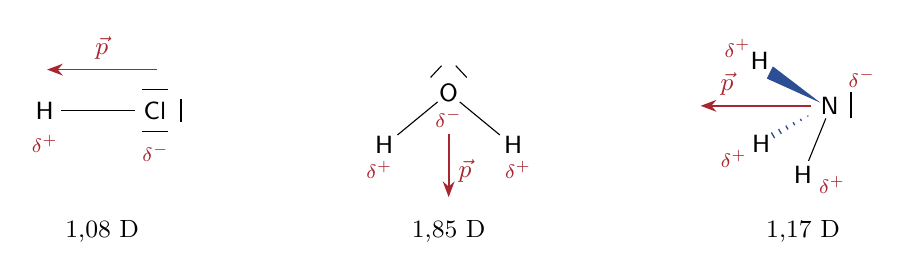
\begin{tikzpicture}
% HCl : doublets non liants de Cl et sens du moment.
\begin{scope}[shift={(0,0)}]
\node[atome]at(-.73,.12){H};\node[atome]at(.67,.12){Cl};\draw(-.52,.12)--(.42,.12);
\draw(.50,.39)--(.84,.39)(.50,-.15)--(.84,-.15)(1.00,-.02)--(1.00,.27);
\node[petit,rougechamp]at(-.73,-.30){$\delta^+$};\node[petit,rougechamp]at(.68,-.42){$\delta^-$};
\draw[echamp](.69,.64)--(-.70,.64)node[midway,above]{$\mom$};
\node at(0,-1.42){$1{,}08~\mathrm D$};
\end{scope}
% Eau : H et H du côté positif.
\begin{scope}[shift={(4.4,0)}]
\node[atome]at(0,.35){O};\draw(-.23,.54)--(-.09,.69)(.09,.69)--(.23,.54);
\draw(-.14,.23)--(-.65,-.19)(.14,.23)--(.65,-.19);
\node[atome]at(-.82,-.32){H};\node[atome]at(.82,-.32){H};
\node[petit,rougechamp]at(0,.02){$\delta^-$};
\node[petit,rougechamp]at(-.88,-.63){$\delta^+$};\node[petit,rougechamp]at(.88,-.63){$\delta^+$};
\draw[echamp](0,-.18)--(0,-.98)node[pos=.58,right]{$\mom$};
\node at(0,-1.42){$1{,}85~\mathrm D$};
\end{scope}
% Ammoniac : une liaison en avant, une en arrière, une dans le plan.
\begin{scope}[shift={(8.9,.00)}]
\node[atome]at(.34,.18){N};\draw(.61,.02)--(.61,.35);
\filldraw[bleutrait](.17,.25)--(-.38,.67)--(-.45,.53)--cycle;
\foreach \s in {1,...,6}{\draw[bleutrait,line width=.48pt]
 ({.15-.085*\s},{.10-.055*\s})--++({-.007*\s},{.012*\s});}
\draw(.29,.02)--(.07,-.52);
\node[atome]at(-.55,.75){H};\node[atome]at(-.53,-.30){H};\node[atome]at(0,-.70){H};
\node[petit,rougechamp]at(-.83,.91){$\delta^+$};\node[petit,rougechamp]at(-.88,-.49){$\delta^+$};
\node[petit,rougechamp]at(.37,-.82){$\delta^+$};\node[petit,rougechamp]at(.75,.53){$\delta^-$};
\draw[echamp](.10,.18)--(-1.30,.18)node[pos=.76,above]{$\mom$};
\node at(0,-1.42){$1{,}17~\mathrm D$};
\end{scope}
\end{tikzpicture}}\label{err:nh}
\end{exemple}
\subsubsection{Dipôle induit}\label{sec:induit}
Un dipôle peut être induit par influence.

\titr{À l'échelle macroscopique}
\surdeux{.45}{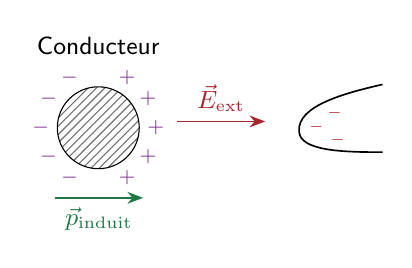
\begin{tikzpicture}
\draw[pattern=north east lines,pattern color=black!55](0,0)circle(.52);
\node[above]at(0,.81){Conducteur};
\foreach \t in {-60,-30,0,30,60}{
 \node[violetdip,font=\scriptsize,inner sep=0pt]at(\t:.73){$+$};
 \node[violetdip,font=\scriptsize,inner sep=0pt]at({180-\t}:.73){$-$};}
\draw[echamp](1.00,.08)--(2.12,.08)node[midway,above]{$\EE$};
\draw[semithick](3.61,.55)..controls(3.13,.44)and(2.53,.28)..(2.55,-.04)
 ..controls(2.55,-.30)and(3.13,-.31)..(3.61,-.31);
\foreach \x/\y in {2.77/.01,3.00/.19,3.04/-.16}
  \node[rougechamp,font=\tiny,inner sep=0pt] at(\x,\y){$-$};
\draw[vvert](-.55,-.89)--(.57,-.89)node[midway,below]{$\vec p_{\mathrm{induit}}$};
\end{tikzpicture}}{Le conducteur est modélisé par un dipôle (cf. complément en fin de cours).}

\titr{Cristal ionique (échelle atomique)}
\fig{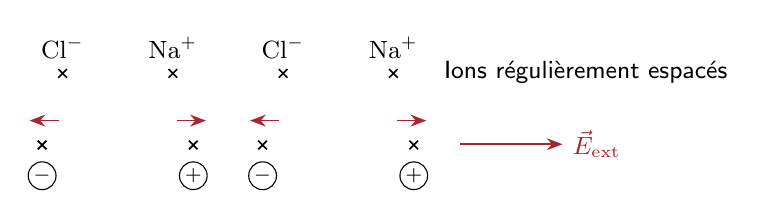
\begin{tikzpicture}
\foreach \x/\s in {0/{\mathrm{Cl}^-},1.4/{\mathrm{Na}^+},2.8/{\mathrm{Cl}^-},4.2/{\mathrm{Na}^+}}{
  \croix{\x}{.7}\node[above] at(\x,.77){$\s$};}
\node[right]at(4.72,.72){Ions régulièrement espacés};
\foreach \x/\sg/\d in {-.26/-/-1,1.66/+/1,2.54/-/-1,4.46/+/1}{
  \croix{\x}{-.21}
  \node[circle,draw,inner sep=.7pt,font=\scriptsize]at(\x,-.6){$\sg$};
  \draw[echamp]({\x-.21*\d},.10)--({\x+.16*\d},.10);}
\draw[echamp](5.05,-.20)--(6.35,-.20)node[right]{$\EE$};
\end{tikzpicture}}
Le déplacement du barycentre des charges crée un dipôle induit.

\titr{Atome}
Dans l'atome d'hydrogène :
\fig{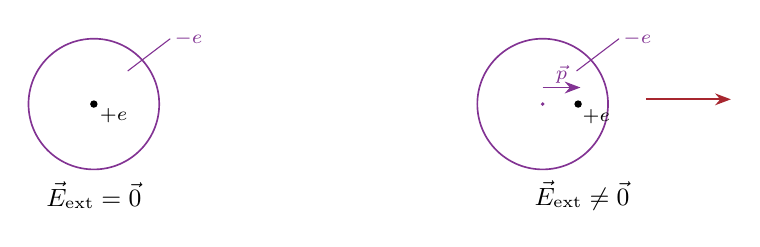
\begin{tikzpicture}
\foreach \k in {0,1}{\begin{scope}[shift={({5.7*\k},0)}]
  \draw[violetdip,semithick](0,0)circle(.83);
  \draw[violetdip,thin](.43,.42)--(.97,.83)node[right,petit]{$-e$};
  \ifnum\k=0
    \fill(0,0)circle(.047);\node[below right,petit]at(.02,0){$+e$};
    \node at(0,-1.16){$\EE=\veczero$};
  \else
    \fill[violetdip](0,0)circle(.025);\fill(.45,0)circle(.047);
    \node[below right,petit]at(.45,-.01){$+e$};
    \draw[moment](0,.21)--(.48,.21)node[midway,above,petit]{$\mom$};
    \draw[echamp](1.31,.06)--(2.39,.06);
    \node at(.50,-1.16){$\EE\ne\veczero$};
  \fi
\end{scope}}
\end{tikzpicture}}
\[\vec p_{\mathrm{induit}}=\alpha\eps\,\EE,\qquad
  \alpha\ \text{est la polarisabilité.}\]
Le dipôle peut être associé à de nombreux systèmes dans la nature, à différentes échelles.
Un dipôle est \textbf{globalement neutre}.

\titr{Différents points de vue}
\begin{itemize}
\item Un \textbf{dipôle actif} est considéré comme une distribution de charges qui crée un champ (partie II).
\item Un \textbf{dipôle passif} subit une action (partie III).
\end{itemize}

% Manuscrit, pages 5 à 8.
\section{Potentiel et champ créés par un dipôle}\label{sec:creation}
\subsection{Considérations de symétrie}\label{sec:sym}
\surdeux{.45}{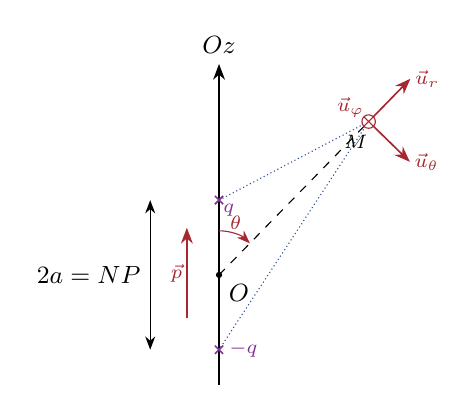
\begin{tikzpicture}[scale=.95]
 \coordinate(O)at(0,0);\coordinate(P)at(0,1);\coordinate(N)at(0,-1);\coordinate(M)at(2.0,2.05);
 \draw[fl](0,-1.47)--(0,2.82)node[above]{$Oz$};
 \draw[bleutrait,densely dotted](P)--(M)--(N);\draw[dashed](O)--(M);
 \fill(O)circle(.042)node[below right]{$O$};
 \croix[violetdip]{0}{1}\croix[violetdip]{0}{-1}
 \node[violetdip,below right,petit]at(P){$q$};\node[violetdip,right,petit]at(.08,-1){$-q$};
 \draw[<->,thin](-.92,-1)--(-.92,1)node[midway,left]{$2a=NP$};
 \draw[echamp](-.43,-.58)--(-.43,.63)node[pos=.5,left,petit]{$\mom$};
 \draw[rougechamp,thin,->](90:.59)arc(90:45.7:.59)node[midway,above,petit]{$\theta$};
 \draw[echamp](M)--++(45.7:.8)node[right,petit]{$\ur$};
 \draw[echamp](M)--++(-44.3:.77)node[right,petit]{$\ut$};
 \draw[rougechamp,fill=white](M)circle(.09);\draw[rougechamp]($(M)+(-.063,-.063)$)--($(M)+(.063,.063)$)
  ($(M)+(-.063,.063)$)--($(M)+(.063,-.063)$);
 \node[rougechamp,above left,petit]at(M){$\uphi$};\node[below left,petit]at(2.04,1.93){$M$};
\end{tikzpicture}}{On utilise la \textbf{base sphérique}, et non la base cylindrique. Son centre \(O\) est le milieu de \(NP\).
\[
\E(M)\ \trois{E_r(r,\theta,\varphi)}{E_\theta(r,\theta,\varphi)}{E_\varphi(r,\theta,\varphi)},
\qquad V(r,\theta,\varphi).
\]}
La distribution est invariante par rotation autour de \((Oz)\). Il en résulte :
\bmath{V(M)=V(r,\theta).}
\bmath{\E=-\grad V=E_r(r,\theta)\,\ur+E_\theta(r,\theta)\,\ut.}
Par symétrie, le plan \((M,\ur,\ut)\) est un plan de symétrie de la distribution \(\D\), donc de \(\E\).
Ainsi, \(\E(M)\in(M,\ur,\ut)\).

\titr{Sur les axes cartésiens}
\surdeux{.41}{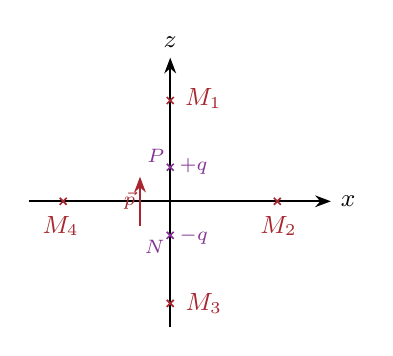
\begin{tikzpicture}[scale=.80]
 \draw[fl](-2.25,0)--(2.55,0)node[right]{$x$};
 \draw[fl](0,-2.0)--(0,2.28)node[above]{$z$};
 \foreach \x/\y/\i in {0/1.60/1,1.7/0/2,0/-1.62/3,-1.70/0/4}{\croix[rougechamp]{\x}{\y}}
 \node[rougechamp,right]at(.08,1.63){$M_1$};\node[rougechamp,below]at(1.72,-.08){$M_2$};
 \node[rougechamp,right]at(.09,-1.62){$M_3$};\node[rougechamp,below]at(-1.74,-.08){$M_4$};
 \croix[violetdip]{0}{.54}\croix[violetdip]{0}{-.54}
 \node[petit,violetdip,above left]at(-.02,.55){$P$};\node[petit,violetdip,right]at(.08,.55){$+q$};
 \node[petit,violetdip,below left]at(-.02,-.55){$N$};\node[petit,violetdip,right]at(.08,-.55){$-q$};
 \draw[echamp](-.48,-.39)--(-.48,.39)node[pos=.52,left,petit]{$\mom$};
\end{tikzpicture}}{Le plan \((Oxy)\) est un plan d'antisymétrie de \(\D\), donc de \(\E\).
Comme \(M_2,M_4\in(Oxy)\),
\[\E(M_2)\parallel(Oz),\qquad \E(M_4)\parallel(Oz).\]
Tous les plans passant par \((Oz)\) sont des plans de symétrie de \(\D\), donc de \(\E\).
Comme \(M_1,M_3\in(Oz)\),
\[\E(M_1)\parallel(Oz),\qquad \E(M_3)\parallel(Oz).\]}

% Manuscrit, pages 8 à 12.
\subsection{Potentiel créé par le dipôle}\label{sec:pot}
Par le théorème de superposition,
\[
 V(M)=\frac{q}{4\pi\eps\,PM}-\frac{q}{4\pi\eps\,NM}.
\]
Pour obtenir le champ, on privilégie la méthode \(\E=-\grad V\).
En effet, l'expression
\[
 \E(M)=\frac{q\,\fle{PM}}{4\pi\eps\,PM^3}
       -\frac{q\,\fle{NM}}{4\pi\eps\,NM^3}
\]
ferait intervenir une somme de vecteurs que l'on souhaite éviter. Le potentiel s'écrit donc :
\bmath{V(M)=\frac{q}{4\pi\eps}\left(\frac1{PM}-\frac1{NM}\right).}
\begin{result}[3]\textbf{Approximation dipolaire}\par
Le point d'observation est loin de la distribution de charges :
\[OM=r\gg a.\]\end{result}
\remaq hors de l'approximation dipolaire, le calcul du potentiel s'arrête à son expression exacte
(cf. carte de champ du chapitre B3).

Dans la suite, on se place dans l'approximation dipolaire (\(r\gg a\)).
\begin{align*}
 \fle{PM}&=\fle{PO}+\fle{OM},\\
 PM^2&=(\fle{PO}+\fle{OM})\cdot(\fle{PO}+\fle{OM})\\
     &=a^2+r^2+2ra\cos\theta,\\
 PM^2&=r^2\left(1+\frac{a^2}{r^2}-2\,\frac ar\cos\theta\right).
\end{align*}
\label{err:pm}
Un développement limité à l'ordre 1 en \(a/r\ll1\) donne
\[
 \frac1{PM}=\frac1r\left(1+\frac{a^2}{r^2}-\frac{2a}r\cos\theta\right)^{-1/2}
 \simeq\frac1r\left(1+\frac ar\cos\theta+\cdots\right).
\]
De même,
\[
 NM^2=a^2+r^2+2ra\cos\theta,\qquad
 \frac1{NM}\simeq\frac1r\left(1-\frac ar\cos\theta+\cdots\right).
\]
Ainsi,
\begin{align*}
 V(M)&=\frac{q}{4\pi\eps}
 \left[\frac1r+\frac a{r^2}\cos\theta-\frac1r+\frac a{r^2}\cos\theta+\cdots\right]\\
 &=\frac{q}{4\pi\eps}\left[
 \underbrace{0}_{\text{ordre 0 en }a/r}
 +\underbrace{\frac{2a}{r^2}\cos\theta}_{\text{ordre 1 en }a/r}+\cdots\right].
\end{align*}
À l'ordre 0, les deux charges se compensent car elles sont opposées. Le terme d'ordre 1
est le terme de plus bas ordre non nul : il est proportionnel à \(1/r^2\).
Le potentiel de cette distribution neutre décroît donc très vite.
\[
 V(M)=\frac{2aq\cos\theta}{4\pi\eps r^2}.
\]
\betoile{5}{V(M)=\frac{p\cos\theta}{4\pi\eps r^2}.}
La référence du potentiel est \(V(r\to+\infty)=0\).

\titr{Formule intrinsèque}
\betoile{4}{V(M)=\frac{\mom\cdot\ur}{4\pi\eps r^2}.}
\titr{Remarques}
\begin{itemize}
\item Le potentiel décroît en \(1/r^2\).
\item Le potentiel est anisotrope : \(V(r,\theta)\) dépend de \(\theta\).
\item Le potentiel est entièrement déterminé par \(\mom\).
\end{itemize}

% Manuscrit, pages 12 à 16.
\subsection{Champ \texorpdfstring{\(\E\)}{E} créé par \texorpdfstring{\(\mom\)}{p}}\label{sec:champ}
\surdeux{.37}{\(\displaystyle
 \E=-\grad V=\left|\begin{matrix}
 -\dfrac{\partial V}{\partial r}\\[4pt]
 -\tfrac1r\,\dfrac{\partial V}{\partial\theta}\\[4pt]
 -\tfrac1{r\sin\theta}\,\dfrac{\partial V}{\partial\varphi}
 \end{matrix}\right..\)}{
\betoile{4}{\E=\frac{p}{4\pi\eps r^3}\,\trois{2\cos\theta}{\sin\theta}{0}.}}
\titr{Formulation intrinsèque}
\[
 \E=\frac{p}{4\pi\eps r^3}\left(2\cos\theta\,\ur+\sin\theta\,\ut\right).
\]
Or, \(\mom=p\cos\theta\,\ur-p\sin\theta\,\ut\). On en déduit
\[
 p\cos\theta=\mom\cdot\ur,\qquad
 p\sin\theta\,\ut=p\cos\theta\,\ur-\mom.
\]
Par conséquent,
\[
 \E(M)=\frac1{4\pi\eps r^3}\left[
 \underbrace{2(\mom\cdot\ur)\ur+p\cos\theta\,\ur}_{3(\mom\cdot\ur)\ur}
 -\mom\right].
\]
\begin{result}[3]
\[
 \E(M)=\frac{1}{4\pi\eps r^5}\big[3(\mom\cdot\vec r)\vec r-r^2\mom\big],
 \qquad \vec r=r\,\ur=\fle{OM}.
\]
\[V(M)=\frac{\mom\cdot\vec r}{4\pi\eps r^3}.\]
\end{result}
\titr{Remarques}
\begin{itemize}
\item Le champ est anisotrope : \(\E(r,\theta)\) dépend de \(\theta\).
\item Le champ électrique est entièrement déterminé par \(\mom\).
\item Le potentiel décroît en \(1/r^2\) et le champ en \(1/r^3\) : la décroissance est beaucoup plus rapide que pour une charge ponctuelle.
\item Dans les exercices, on privilégiera la formule en coordonnées sphériques. La formulation intrinsèque peut servir dans certains cas, notamment pour les interactions dipôle-dipôle.
\end{itemize}
\surdeux{.45}{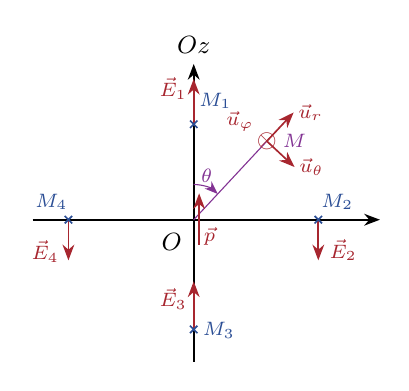
\begin{tikzpicture}[scale=.86]
 \draw[fl](-2.38,0)--(2.75,0);\draw[fl](0,-2.1)--(0,2.30)node[above]{$Oz$};
 \draw[violetdip](0,0)--(1.08,1.16);\draw[violetdip,->](90:.52)arc(90:47:.52)node[midway,above,petit]{$\theta$};
 \draw[echamp](1.08,1.16)--++(47:.58)node[right,petit]{$\ur$};
 \draw[echamp](1.08,1.16)--++(-43:.56)node[right,petit]{$\ut$};
 \node[rougechamp,inner sep=0pt,font=\small] at(1.08,1.16){$\otimes$};
 \node[rougechamp,above left,petit]at(.95,1.24){$\uphi$};
 \node[violetdip,right,petit]at(1.25,1.16){$M$};\node[below left]at(-.03,-.06){$O$};
 \draw[echamp](.08,-.37)--(.08,.39)node[pos=.17,right,petit]{$\mom$};
 \foreach \x/\y/\dy/\i in {0/1.41/.67/1,1.84/0/-.60/2,0/-1.62/.71/3,-1.85/0/-.60/4}{
   \draw[echamp](\x,\y)--++(0,\dy);\croix[bleutrait]{\x}{\y}}
 \node[bleutrait,above right,petit]at(.02,1.57){$M_1$};\node[rougechamp,left,petit]at(-.04,1.94){$\vec E_1$};
 \node[bleutrait,above right,petit]at(1.82,.08){$M_2$};\node[rougechamp,right,petit]at(1.94,-.45){$\vec E_2$};
 \node[bleutrait,right,petit]at(.07,-1.63){$M_3$};\node[rougechamp,left,petit]at(-.04,-1.17){$\vec E_3$};
 \node[bleutrait,above left,petit]at(-1.80,.08){$M_4$};\node[rougechamp,left,petit]at(-1.93,-.47){$\vec E_4$};
\end{tikzpicture}}{\[
\begin{aligned}
 M_1:\ \theta&=0,& \E&=\tfrac{p}{4\pi\eps r^3}\,\trois{2}{0}{0};\\[3pt]
 M_3:\ \theta&=\pi,& \E&=\tfrac{p}{4\pi\eps r^3}\,\trois{-2}{0}{0};\\[3pt]
 M_2,M_4:\ \theta&=\tfrac\pi2,& \E&=\tfrac{p}{4\pi\eps r^3}\,\trois{0}{1}{0}.
\end{aligned}\]}

% Manuscrit, pages 16 à 18.
\subsection{Carte de champ}\label{sec:carte}
\[
 V(M)=\frac{p\cos\theta}{4\pi\eps r^2},\qquad
 \E=\frac p{4\pi\eps r^3}\,\trois{2\cos\theta}{\sin\theta}{0}.
\]
\Needspace{42mm}
\titr{Surfaces équipotentielles}
\[
 V(M)=\cste\quad\Longleftrightarrow\quad \frac{\cos\theta}{r^2}=\cste'.
\]
\begin{cadre}
\[r^2=K\cos\theta.\]
Le rayon \(r\) est maximal pour \(\theta=0\) et nul pour \(\theta=\pi/2\).
\end{cadre}
\titr{Lignes de champ de \texorpdfstring{\(\E\)}{E}}
\[
 \frac{\dd r}{E_r}=\frac{r\,\dd\theta}{E_\theta}
 \quad\Longleftrightarrow\quad
 \frac{\dd r}{2\cos\theta}=\frac{r\,\dd\theta}{\sin\theta}
 \quad\Longleftrightarrow\quad
 \frac{2\cos\theta}{\sin\theta}\,\dd\theta=\frac1r\,\dd r.
\]
En intégrant, on obtient \(\ln|r|=2\ln|\sin\theta|+\cste''\).
\begin{cadre}
\[r=K'\sin^2\theta.\]
Le rayon \(r\) est nul pour \(\theta=0\) et maximal pour \(\theta=\pi/2\).
\end{cadre}

\fig{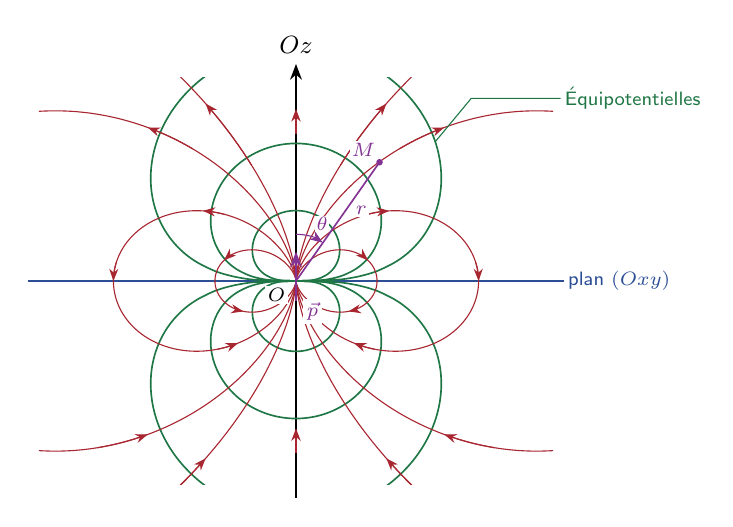
\begin{tikzpicture}[x=1.04cm,y=1.04cm]
 % Section méridienne : vert, r^2 = K cos(theta) ; rouge, r = K' sin^2(theta).
 \draw[bleutrait,thin](-3.27,0)--(3.27,0) node[right,petit]{plan $(Oxy)$};
 \draw[fl](0,-2.65)--(0,2.65) node[above]{$Oz$};
 \begin{scope}
  \clip(-3.14,-2.48) rectangle(3.14,2.48);
  \foreach \haut in {-1,1}{\foreach \k in {.86,1.68,2.86}{
   \draw[vertequi,semithick,smooth,domain=-90:90,samples=105,variable=\t]
   plot ({\k*sqrt(max(0,cos(\t)))*sin(\t)},{\haut*\k*(max(0,cos(\t)))^1.5});
  }}
  \foreach \bord in {-1,1}{\foreach \k/\angles in {.99/{74,120},2.23/{53,90,137},5.4/{44,136},11.8/{27,153}}{
   \draw[rougechamp,thin] plot[domain=0:180,samples=100,smooth,variable=\t]
      ({\bord*\k*sin(\t)^3},{\k*sin(\t)^2*cos(\t)});
   \foreach \tmark in \angles {\pgfmathsetmacro{\tstart}{\tmark-6}
    \draw[rougechamp,thin,-{Stealth[length=1.55mm,width=1.15mm]}] plot[domain=\tstart:\tmark,samples=5,smooth,variable=\t]
      ({\bord*\k*sin(\t)^3},{\k*sin(\t)^2*cos(\t)});}
  }}
 \end{scope}
 \draw[rougechamp,-{Stealth[length=1.6mm]}](0,1.80)--(0,2.10);
 \draw[rougechamp,-{Stealth[length=1.6mm]}](0,-2.10)--(0,-1.80);
 \draw[moment](0,-.24)--(0,.36);
 \node[left,petit,fill=white,inner sep=1pt]at(-.09,-.17){$O$};
 \node[violetdip,petit,below right,fill=white]at(.08,-.21){$\mom$};
 \draw[violetdip,semithick](0,0)--(1.02,1.45);
 \fill[violetdip](1.02,1.45)circle(.04);
 \node[violetdip,above left,petit,fill=white,inner sep=.8pt]at(1.00,1.49){$M$};
 \node[violetdip,right,petit,fill=white,inner sep=1pt]at(.69,.86){$r$};
 \draw[violetdip,->,thin](90:.57)arc(90:55:.57);
 \node[violetdip,petit,fill=white,inner sep=.5pt]at(.32,.70){$\theta$};
 \draw[vertequi,thin] (1.7006,1.7006)--(2.14,2.23)--(3.23,2.23);
 \node[vertequi,right,petit]at(3.23,2.23){Équipotentielles};
\end{tikzpicture}}

\titr{Remarques}
\begin{itemize}
\item Le plan du tableau est un plan de symétrie de \(\D\), donc de \(\E\).
\item Le plan \((Oxy)\) est un plan d'antisymétrie de \(\D\), donc de \(\E\).
Le champ \(\E\) coupe ce plan perpendiculairement.
\item Le plan \((Oyz)\) est un plan de symétrie de \(\D\), donc de \(\E\).
\item Les lignes de champ semblent fermées. En réalité, les expressions obtenues ne sont valables que loin du dipôle.
\end{itemize}

% Manuscrit, pages 19 à 22.
\section{Actions subies par un dipôle dans un champ extérieur}\label{sec:actions}
Dans cette partie, on fait abstraction du champ électrique créé par le dipôle lui-même.
On place le dipôle dans un champ électrique extérieur \(\EE\), créé par une distribution statique \(\D\).

\surdeux{.29}{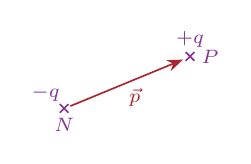
\begin{tikzpicture}
 \croix[violetdip]{-.80}{-.33}\croix[violetdip]{.8}{.33}
 \draw[echamp](-.72,-.30)--(.71,.29)node[pos=.48,below right,petit]{$\mom$};
 \node[violetdip,above left,petit]at(-.80,-.29){$-q$};\node[violetdip,below,petit]at(-.80,-.40){$N$};
 \node[violetdip,above,petit]at(.80,.39){$+q$};\node[violetdip,right,petit]at(.89,.32){$P$};
\end{tikzpicture}}{\textbf{Système :} le dipôle de moment \(\mom\), constitué des charges \(\{-q,q\}\).

\textbf{Actions :}
\begin{itemize}
\item La force résultante est \(\FR=-q\,\EE(N)+q\,\EE(P)\).
\item Le moment résultant en \(A\) est
\(\vec M_A^{\,\text{rés}}=\fle{AN}\wedge[-q\,\EE(N)]+\fle{AP}\wedge q\,\EE(P)\).
\end{itemize}}

\subsection{Actions dans un champ uniforme}\label{sec:uniforme}
\begin{exemple}\examtitle{Exemple}
On place le dipôle dans un condensateur plan.
\fig{\begin{tikzpicture}
 \draw[vertequi,dashed](-.88,-.52)--(.88,.52);\fill[vertequi](0,0)circle(.04);
 \node[vertequi,below right,petit]at(.03,-.06){$O$};
 \croix[violetdip]{-.88}{-.52}\croix[violetdip]{.88}{.52}
 \node[violetdip,above left,petit]at(-.88,-.47){$N$};\node[violetdip,below,petit]at(-.88,-.60){$-q$};
 \node[violetdip,above,petit]at(.88,.59){$P$};\node[violetdip,below,petit]at(.94,.46){$+q$};
 \draw[echamp](-.94,-.52)--(-2.30,-.52)node[midway,below]{$\vec F_N$};
 \draw[echamp](.94,.52)--(2.30,.52)node[midway,above]{$\vec F_P$};
 \draw[echamp](2.60,-.45)--(3.58,-.45)node[right]{$\EE$};
\end{tikzpicture}}
\end{exemple}
\[\FR=q\,\EE-q\,\EE.\]
\betoile{4}{\FR=\veczero.}
Le centre d'inertie \(O\) du dipôle reste fixe. Le dipôle subit un \textbf{couple}.\label{err:repos}

\textbf{Rappel :} pour un couple, \(\vec M_A\) est indépendant de \(A\).
Par rapport à \(O\),
\begin{align*}
 \MR&=\fle{OP}\wedge q\,\EE+\fle{ON}\wedge(-q\,\EE)\\
 &=q(\fle{OP}-\fle{ON})\wedge\EE
 =q\,\fle{NP}\wedge\EE.
\end{align*}
\betoile{4}{\MR=\mom\wedge\EE.}
Le dipôle tourne sur lui-même.

\titr{Équilibre}
\[
 \vec M_O=\veczero\quad\Longleftrightarrow\quad\mom\parallel\EE.
\]
Le dipôle est donc à l'équilibre lorsque \(\mom\) et \(\EE\) sont colinéaires.
\fig{\begin{minipage}[t]{.47\linewidth}\centering
 \equilibrefig{37}\par
 Si \(\mom\) et \(\E\) sont de même sens,\\ l'équilibre est \textbf{stable}.
 \end{minipage}\hfill\begin{minipage}[t]{.47\linewidth}\centering
 \equilibrefig{134}\par
 Si \(\mom\) et \(\E\) sont de sens opposés,\\ l'équilibre est \textbf{instable}.
 \end{minipage}}
\begin{result}[4]
Dans un champ extérieur uniforme, le dipôle subit un couple de forces qui tend à aligner son moment dipolaire avec \(\E\), dans le même sens.
Le dipôle dans son ensemble ne se déplace pas : son centre d'inertie reste fixe.
\end{result}
\surdeux{.37}{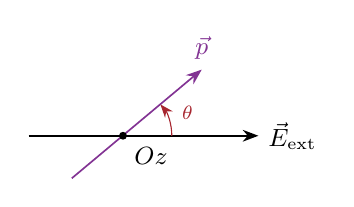
\begin{tikzpicture}
 \draw[fl](-1.20,0)--(1.72,0)node[right]{$\EE$};
 \draw[moment](-.65,-.54)--(1.00,.84)node[above]{$\mom$};
 \fill(0,0)circle(.05);\node[below right]at(.02,-.03){$Oz$};
 \draw[rougechamp,->](.62,0)arc(0:40:.62);
 \node[petit,rougechamp]at(.82,.29){$\theta$};
\end{tikzpicture}}{Le théorème du moment cinétique, appliqué à l'axe \((Oz)\) fixe dans le référentiel galiléen, donne
\[J\ddot\theta=-p\,\EEsc\sin\theta.\]
Le mouvement est oscillatoire.}

% Manuscrit, pages 22 à 26.
\subsection{Actions dans un champ non uniforme}\label{sec:variable}
\fig{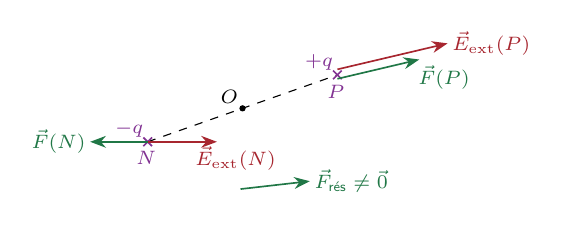
\begin{tikzpicture}
 \coordinate(N)at(-1.48,-.39);\coordinate(P)at(.93,.46);
 \draw[dashed](N)--(P);\fill(-.275,.035)circle(.04)node[above left,petit]{$O$};
 \croix[violetdip]{-1.48}{-.39}\croix[violetdip]{.93}{.46}
 \node[violetdip,above left,petit]at(N){$-q$};\node[violetdip,below,petit]at(-1.5,-.46){$N$};
 \node[violetdip,above left,petit]at(P){$+q$};\node[violetdip,below,petit]at(.91,.39){$P$};
 \draw[echamp](N)--++(.88,0)node[pos=.62,below right,petit]{$\EE(N)$};
 \draw[vvert](N)--++(-.73,0)node[left,petit]{$\vec F(N)$};
 \draw[echamp](.93,.53)--++(1.4,.33)node[right,petit]{$\EE(P)$};
 \draw[vvert](.93,.41)--++(1.04,.245)node[pos=.93,below right,petit]{$\vec F(P)$};
 \draw[vvert](-.30,-.99)--(.58,-.89)node[right,petit]{$\FR\ne\veczero$};
\end{tikzpicture}}
\[\FR=q\,\EE(P)-q\,\EE(N)\ne\veczero.\]

\Needspace{47mm}
\titr{Approximation}
La taille \(2a\) du dipôle est petite devant la distance caractéristique \(L\) de variation de \(\EE\) :
\(2a\ll L\). On effectue un développement limité en \(a/L\).
On développe en série de Taylor autour de \(O\) le champ vectoriel à trois variables \(\EE(x,y,z)\).
\begin{align*}
 E_x(x,y,z)={}&E_x(x_0,y_0,z_0)+(x-x_0)\left.\frac{\partial E_x}{\partial x}\right|_O\\
 &+(y-y_0)\left.\frac{\partial E_y}{\partial y}\right|_O
  +(z-z_0)\left.\frac{\partial E_z}{\partial z}\right|_O .
\end{align*}
\label{err:taylor}
On procède de même pour \(E_y(x,y,z)\) et \(E_z(x,y,z)\) :
\[
 \left\{\begin{aligned}
 E(x,y,z)&=E_x(x_0,y_0,z_0)+\big(\fle{OM}\cdot\grad\big)_O E_x,\\
 E_y(x,y,z)&=E_y(x_0,y_0,z_0)+\big(\fle{OM}\cdot\grad\big)_O E_y,\\
 E_z(x,y,z)&=E_z(x_0,y_0,z_0)+\big(\fle{OM}\cdot\grad\big)_O E_z .
 \end{aligned}\right.
\]
\bmath{\E(M)=\E(O)+\big(\fle{OM}\cdot\grad\big)_O\,\EE.}
La résultante des forces s'écrit alors
\begin{align*}
 \FR&=q\,\EE(P)-q\,\EE(N)\\
 &=q\left[\EE(O)+(\fle{OP}\cdot\grad)_O\EE
       -\EE(O)-(\fle{ON}\cdot\grad)_O\EE\right]\\
 &=q\left[\underbrace{\veczero}_{\text{ordre 0 en }a/L}
      +\underbrace{(\fle{NP}\cdot\grad)_O\EE}_{\text{ordre 1 en }a/L}\right].
\end{align*}
\betoile{4}{\FR=(\mom\cdot\grad)_O\,\EE.}
La résultante est d'ordre 1 en \(a/L\). Le dipôle se déplace car \(\FR\ne\veczero\).

Pour le moment résultant, on conserve l'ordre 0, le plus bas ordre non nul du développement du champ :
\begin{align*}
 \MR&=\fle{OP}\wedge q\,\EE(P)-\fle{ON}\wedge q\,\EE(N)\\
 &=\fle{OP}\wedge q\,\EE(O)-\fle{ON}\wedge q\,\EE(O)
 =q\,\fle{NP}\wedge\EE(O).
\end{align*}
\betoile{4}{\MR=\mom\wedge\EE(O).}
Cette expression est d'ordre 0 en \(a/L\).

\surdeux{.32}{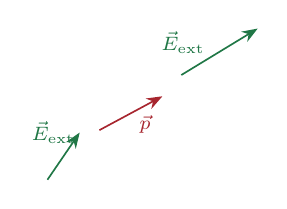
\begin{tikzpicture}
 \draw[vvert](-1.0,-.65)--(-.59,-.05)node[left,petit]{$\EE$};
 \draw[echamp](-.34,-.02)--(.46,.41)node[pos=.56,below right,petit]{$\mom$};
 \draw[vvert](.70,.68)--(1.67,1.27)node[pos=.37,above left,petit]{$\EE$};
\end{tikzpicture}}{Le dipôle subit un moment résultant et une force résultante.
Le moment résultant l'emporte (ordre 0 contre ordre 1) : dans un premier temps, le dipôle tend à s'aligner avec le champ.}

\surdeux{.49}{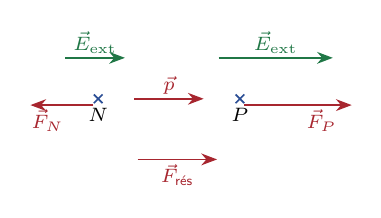
\begin{tikzpicture}
 \croix[bleutrait]{-.90}{0}\croix[bleutrait]{.90}{0}
 \node[below,petit]at(-.9,-.07){$N$};\node[below,petit]at(.9,-.07){$P$};
 \draw[vvert](-1.32,.52)--(-.56,.52)node[midway,above,petit]{$\EE$};
 \draw[vvert](.63,.52)--(2.08,.52)node[midway,above,petit]{$\EE$};
 \draw[echamp](-.44,0)--(.44,0)node[midway,above,petit]{$\mom$};
 \draw[echamp](-.96,-.08)--(-1.76,-.08)node[pos=.73,below,petit]{$\vec F_N$};
 \draw[echamp](.95,-.08)--(2.32,-.08)node[pos=.72,below,petit]{$\vec F_P$};
 \draw[echamp](-.40,-.77)--(.61,-.77)node[midway,below,petit]{$\FR$};
\end{tikzpicture}}{Le dipôle subit une force qui le conduit vers une zone où la norme de \(\EE\) est forte.}
\begin{result}[4]
Dans un champ électrique non uniforme, le dipôle subit principalement un moment qui tend
à l'aligner avec le champ électrique, dans le même sens. Une fois aligné, le dipôle subit une force qui tend à le déplacer vers la zone de champ le plus fort.
\end{result}

% Manuscrit, pages 27 à 30.
\fig{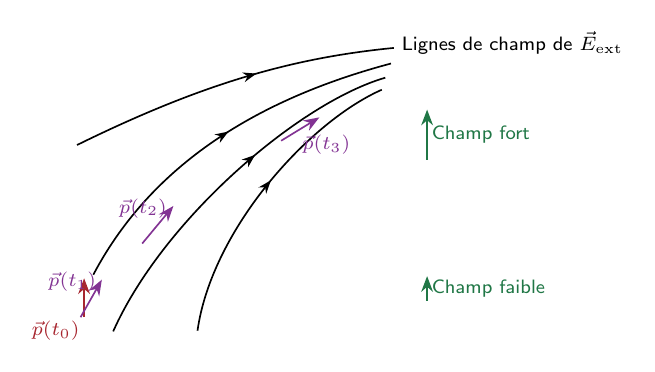
\begin{tikzpicture}[scale=.90]
 \draw[semithick,sens=.58](-2.30,.70)..controls(-.55,1.56)and(.73,1.93)..(2.17,2.07);
 \draw[semithick,sens=.53](-2.07,-1.13)..controls(-1.20,.52)and(.40,1.39)..(2.13,1.85);
 \draw[semithick,sens=.60](-1.79,-1.93)..controls(-1.08,-.34)and(.84,1.30)..(2.05,1.65);
 \draw[semithick,sens=.54](-.60,-1.92)..controls(-.40,-.50)and(.96,1.02)..(2.00,1.48);
 \draw[echamp](-2.2,-1.73)--(-2.2,-1.18)node[pos=.03,below left,petit]{$\mom(t_0)$};
 \draw[moment](-2.25,-1.73)--(-1.95,-1.20)node[pos=.95,left,petit]{$\mom(t_1)$};
 \draw[moment](-1.38,-.69)--(-.94,-.16)node[pos=.94,left,petit]{$\mom(t_2)$};
 \draw[moment](.58,.76)--(1.12,1.09)node[pos=.43,below right,petit]{$\mom(t_3)$};
 \node[petit,above right]at(2.22,1.92){Lignes de champ de $\EE$};
 \draw[vvert](2.64,.49)--(2.64,1.20)node[midway,right,petit]{Champ fort};
 \draw[vvert](2.64,-1.50)--(2.64,-1.15)node[midway,right,petit]{Champ faible};
\end{tikzpicture}}

\begin{exemple}\examtitle{Déviation d'un jet d'eau}
\fig{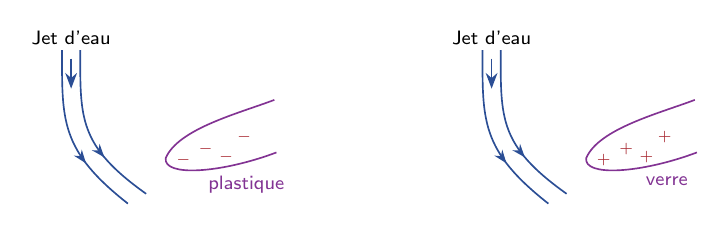
\begin{tikzpicture}[scale=.89]
 \foreach \x/\mat/\sg in {0/plastique/-,6/verre/+}{\begin{scope}[shift={(\x,0)}]
 \draw[bleutrait,semithick,sens=.67](-1.12,1.17)..controls(-1.12,.17)and(-1.15,-.26)..(-.18,-1.02);
 \draw[bleutrait,semithick,sens=.67](-.86,1.17)..controls(-.86,.20)and(-.89,-.19)..(.08,-.88);
 \draw[bleutrait,fl](-.99,1.05)--(-.99,.62);
 \node[above,petit]at(-.99,1.18){Jet d'eau};
 \draw[violetdip,semithick](1.91,.46)..controls(1.41,.27)and(.54,.05)..(.36,-.37)
 ..controls(.32,-.64)and(1.14,-.59)..(1.94,-.29);
 \foreach \xx/\yy in {.61/-.40,.93/-.24,1.22/-.36,1.48/-.07}
 \node[rougechamp,font=\tiny,inner sep=0pt]at(\xx,\yy){$\sg$};
 \node[violetdip,below,petit]at(1.51,-.57){\mat};
 \end{scope}}
\end{tikzpicture}}
La molécule d'eau \(\mathrm{H_2O}\) possède un moment dipolaire \(\mom\).
\fig{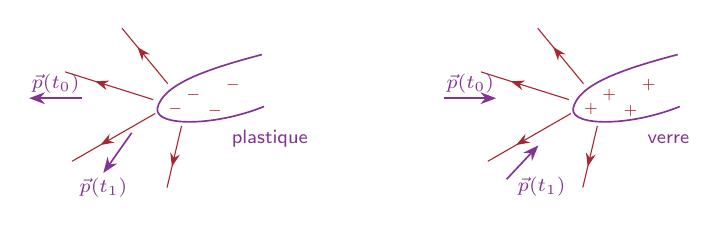
\begin{tikzpicture}[scale=.88]
 \foreach \x/\mat/\sg in {0/plastique/-,6/verre/+}{\begin{scope}[shift={(\x,0)}]
 \draw[violetdip,semithick](1.85,.61)..controls(1.01,.39)and(.41,.17)..(.34,-.17)
 ..controls(.31,-.43)and(1.16,-.43)..(1.88,-.14);
 \foreach \xx/\yy in {.60/-.17,.86/.03,1.17/-.20,1.43/.17}
   \node[rougechamp,font=\tiny,inner sep=0pt]at(\xx,\yy){$\sg$};
 \node[violetdip,right,petit]at(1.35,-.61){\mat};
 \foreach \xstart/\ystart/\xend/\yend in {.49/.19/-.17/.99,.28/-.04/-.99/.36,.31/-.24/-.89/-.93,.69/-.42/.48/-1.31}
   \draw[rougechamp,thin,sens=.66](\xstart,\ystart)--(\xend,\yend);
 \ifdim\x pt=0pt
  \draw[moment](-.75,-.02)--(-1.51,-.02)node[midway,above,petit]{$\mom(t_0)$};
  \draw[moment](-.03,-.52)--(-.44,-1.10)node[below,petit]{$\mom(t_1)$};
 \else
  \draw[moment](-1.52,-.02)--(-.77,-.02)node[midway,above,petit]{$\mom(t_0)$};
  \draw[moment](-.62,-1.19)--(-.16,-.70)node[pos=.20,below right,petit]{$\mom(t_1)$};
 \fi
 \end{scope}}
\end{tikzpicture}}\label{err:jet}
\end{exemple}

\remaq si l'on oblige le dipôle à rester anti-aligné (\(\mom\) et \(\E\) restent de sens opposés),
la situation est la suivante :
\surdeux{.47}{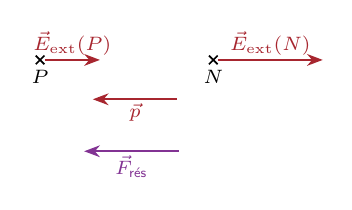
\begin{tikzpicture}
 \croix{-1.16}{.20}\croix{1.04}{.20}
 \node[below,petit]at(-1.16,.12){$P$};\node[below,petit]at(1.04,.12){$N$};
 \draw[echamp](-1.10,.20)--(-.40,.20)node[midway,above,petit]{$\EE(P)$};
 \draw[echamp](1.10,.20)--(2.43,.20)node[midway,above,petit]{$\EE(N)$};
 \draw[echamp](.58,-.30)--(-.49,-.30)node[midway,below,petit]{$\mom$};
 \draw[moment](.60,-.96)--(-.60,-.96)node[midway,below,petit]{$\FR$};
\end{tikzpicture}}{Le dipôle subit une force qui le déplace vers une zone où la norme de \(\EE\) est faible.}

\begin{align*}
 \vec F&=(\mom\cdot\grad)\EE\\
 &=\left(p_x\frac{\partial}{\partial x}+p_y\frac{\partial}{\partial y}
       +p_z\frac{\partial}{\partial z}\right)\EE\\
 &=\left(p_r\frac{\partial}{\partial r}+\frac{p_\theta}{r}\frac{\partial}{\partial\theta}
       +p_z\frac{\partial}{\partial z}\right)\EE\\
 &=\left(p_r\frac{\partial}{\partial r}+\frac{p_\theta}{r}\frac{\partial}{\partial\theta}
       +\frac{p_\varphi}{r\sin\theta}\frac{\partial}{\partial\varphi}\right)\EE .
\end{align*}
Si \(\mom=p_x\ux\) et \(\E=E_x\ux\), alors
\bmath{\vec F=p_x\frac{\partial E_x}{\partial x}\,\ux.}
On retrouve les deux situations : un dipôle aligné avec \(\E\) se dirige vers les champs forts ;
un dipôle anti-aligné avec \(\E\) se dirige vers les champs faibles.

% Manuscrit, pages 30 à 34.
\Needspace{53mm}
\subsection{Énergie potentielle d'interaction d'un dipôle rigide}\label{sec:energie}
\surdeux{.32}{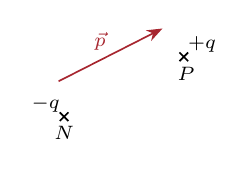
\begin{tikzpicture}
 \croix{-.76}{-.38}\croix{.76}{.38}
 \node[above left,petit]at(-.76,-.38){$-q$};\node[below,petit]at(-.76,-.45){$N$};
 \node[above right,petit]at(.76,.38){$+q$};\node[below,petit]at(.79,.30){$P$};
 \draw[echamp](-.83,.07)--(.49,.74)node[midway,above left,petit]{$\mom$};
\end{tikzpicture}}{\textbf{Système :} les deux charges \(\{-q,q\}\).\par
Le système subit deux forces conservatives.
\[
\begin{aligned}
 E_p&=E_p(N)+E_p(P)\\
    &=-q\,\VE(N)+q\,\VE(P).
\end{aligned}
\]}
\textbf{Hypothèse :}
\begin{itemize}[nosep]\item \(a\ll L\).\end{itemize}
On développe alors les potentiels :
\[
 \begin{aligned}
 \VE(P)&=\VE(O)+\fle{OP}\cdot\grad_O\VE,\\
 \VE(N)&=\VE(O)+\fle{ON}\cdot\grad_O\VE.
 \end{aligned}
\]
Il en résulte
\[
 \begin{aligned}
 E_p&=q\big[0+\fle{OP}\cdot\grad_O\VE-\fle{ON}\cdot\grad_O\VE\big]\\
    &=q\,\fle{NP}\cdot\grad_O\VE.
 \end{aligned}
\]
\betoile{4}{E_p=-\mom\cdot\EE(O).}

\titr{Remarques}
\begin{itemize}
\item On dispose de formules analogues pour les dipôles magnétiques.
\item On peut retrouver tous les résultats précédents à partir de \(E_p=-\mom\cdot\EE(O)\).
Pour minimiser \(E_p\), il faut que \(\mom\) soit aligné avec \(\EE\).
Une fois aligné, le dipôle va vers les zones de champ \(\EE\) faible.\label{err:faible}
\item Considérons le cas où le centre d'inertie \(O\) du dipôle est fixe.
\end{itemize}
\surdeux{.43}{\centering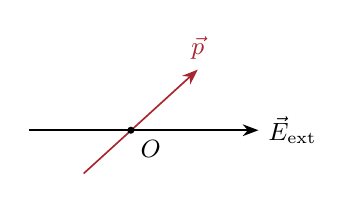
\begin{tikzpicture}
 \draw[fl](-1.30,0)--(1.62,0)node[right]{$\EE$};
 \draw[echamp](-.60,-.55)--(.85,.77)node[above]{$\mom$};
 \fill(0,0)circle(.045)node[below right]{$O$};
\end{tikzpicture}\par\smallskip \(E_p=-p\,\EEsc\cos\theta=E_p(\theta).\)}{
\centering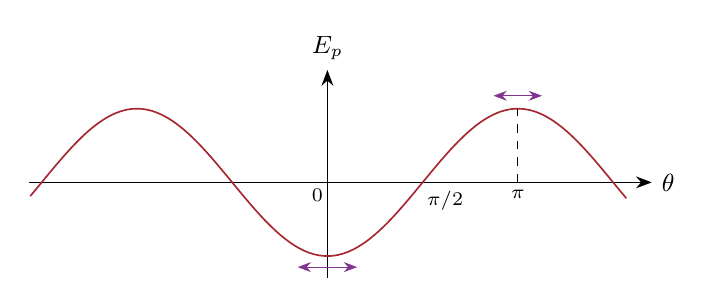
\begin{tikzpicture}[x=.77cm,y=.78cm]
 \draw[fl](-4.93,0)--(5.35,0)node[right]{$\theta$};
 \draw[fl](0,-1.55)--(0,1.83)node[above]{$E_p$};
 \draw[rougechamp,semithick,domain=-4.90:4.93,samples=100,smooth]plot(\x,{-1.20*cos(\x r)});
 \draw[dashed](3.14159,0)--(3.14159,1.20);
 \node[petit,below left]at(0,-.04){$0$};\node[petit,below right]at(1.571,-.06){$\pi/2$};
 \node[petit,below]at(3.142,-.05){$\pi$};
 \draw[violetdip,<->]( -.49,-1.38)--(.49,-1.38);
 \draw[violetdip,<->](2.74,1.41)--(3.54,1.41);
\end{tikzpicture}}
Pour \(\theta=0\ [2\pi]\), l'équilibre est stable. Pour \(\theta=\theta\ [2\pi]\), l'équilibre est instable.\label{err:instable}

On peut montrer que, pour un \textbf{dipôle rigide},
\bmath{\FR=(\mom\cdot\grad)_O\EE=-\grad E_p.}
Cette relation peut être utilisée dans les sujets de concours. Elle n'est pas immédiate :
la formule \(\vec F=-\grad E_p\) est connue pour un point matériel ; ici, il faut la démontrer.
\begin{result}[5]\[\vec F=(\mom\cdot\grad)\EE,\qquad \vec M_O=\mom\wedge\EE(O).\]\end{result}
Ces deux relations sont vraies que le dipôle soit rigide ou induit.
\betoile{5}{E_p=-\mom\cdot\EE(O).}
Cette dernière relation n'est vraie que pour un dipôle \textbf{rigide}.

% Manuscrit, pages 34 à 39.
\section{Applications autour du concept de dipôle}\label{sec:applications}
\subsection{Développement multipolaire}\label{sec:multi}
\surdeux{.48}{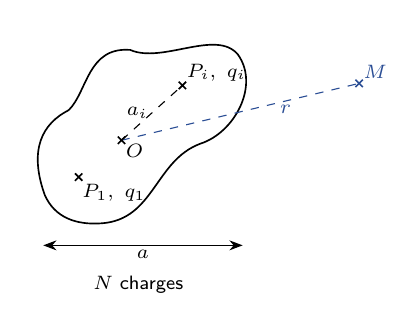
\begin{tikzpicture}[scale=.85]
 \draw[semithick](-1.69,-.78)..controls(-1.93,-.10)and(-1.72,.28)..(-1.33,.48)
 ..controls(-1.05,.75)and(-1.05,1.43)..(-.41,1.38)
 ..controls(.07,1.17)and(.88,1.70)..(1.20,1.31)
 ..controls(1.53,.84)and(1.14,.14)..(.64,-.02)
 ..controls(-.04,-.27)and(-.05,-1.15)..(-.83,-1.21)
 ..controls(-1.21,-1.24)and(-1.54,-1.13)..(-1.69,-.78)--cycle;
 \coordinate(O)at(-.54,.03);\coordinate(I)at(.37,.85);\coordinate(M)at(3.01,.88);
 \draw[dashed](O)--(I)node[midway,left,petit]{$a_i$};
 \draw[bleutrait,dashed](O)--(M)node[pos=.69,below,petit]{$r$};
 \croix{-.54}{.03}\node[below right,petit]at(O){$O$};
 \croix{.37}{.85}\node[above right,petit]at(I){$P_i,\ q_i$};
 \croix{-1.18}{-.52}\node[below right,petit]at(-1.19,-.56){$P_1,\ q_1$};
 \croix[bleutrait]{3.01}{.88}\node[above right,bleutrait,petit]at(M){$M$};
 \draw[<->](-1.71,-1.54)--(1.27,-1.54)node[midway,below,petit]{$a$};
 \node[petit]at(-.29,-2.12){$N$ charges};
\end{tikzpicture}}{On cherche le champ \(\E(M)\) et le potentiel \(V(M)\) à l'aide de l'approximation dipolaire, avec \(a\ll r\).}
\[
 V(M)=\sum_{i=0}^N\frac{q_i}{4\pi\eps\,P_iM}.
\]\label{err:bornes}
Comme \(\fle{P_iM}=\fle{P_iO}+\fle{OM}\), on a
\begin{align*}
 P_iM^2&=a_i^2+r^2-2\vec a_i\cdot\fle{OM}\\
 &=r^2\left(1+\frac{a_i^2}{r^2}-\frac{2\vec a_i\cdot\fle{OM}}{r^2}\right),\\
 \frac{1}{P_iM}
 &=\frac1r\left(1+\frac{a_i^2}{r^2}-\frac{2\vec a_i\cdot\fle{OM}}{r^2}\right)^{-1/2}\\
 &\simeq\frac1r\left[
  \underbrace{1}_{\text{ordre 0 en }a/r}
 +\underbrace{\frac{\vec a_i\cdot\fle{OM}}{r^2}}_{\text{ordre 1 en }a/r}+\cdots\right].
\end{align*}
On obtient
\bmath{V(M)=\frac{\displaystyle\sum_{i=2}^N q_i}{4\pi\eps r}
 +\frac{1}{4\pi\eps r^3}\sum_{i=1}^N q_i\vec a_i\cdot\fle{OM}+\cdots.}
\titr{Premier cas}
Si \(\displaystyle\sum_{i=1}^N q_i=Q\ne0\), la distribution \(\D\) n'est pas neutre :
\[
 V(M)\simeq\frac{Q}{4\pi\eps r}.
\]
\begin{exemple}\examtitle{Exemples}
C'est le cas des ions \(\mathrm{Na^+}\), \(\mathrm{Cl^-}\), \(\mathrm{H_3O^+}\), etc.
Dans l'approximation dipolaire :
\fig{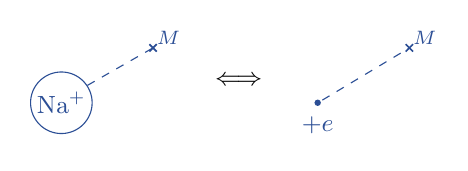
\begin{tikzpicture}[scale=.85]
 \draw[bleutrait](0,0)circle(.46);\node[bleutrait]at(0,0){$\mathrm{Na^+}$};
 \draw[bleutrait,dashed](.39,.26)--(1.37,.82);\croix[bleutrait]{1.37}{.82}
 \node[above right,bleutrait,petit]at(1.36,.80){$M$};
 \node at(2.65,.32){$\Longleftrightarrow$};
 \fill[bleutrait](3.83,0)circle(.048);\node[below,bleutrait]at(3.83,-.06){$+e$};
 \draw[bleutrait,dashed](3.90,.04)--(5.20,.82);\croix[bleutrait]{5.20}{.82}
 \node[above right,bleutrait,petit]at(5.19,.80){$M$};
\end{tikzpicture}}
\end{exemple}
\titr{Deuxième cas}
Si \(\displaystyle\sum_{i=1}^N q_i=0\), la distribution \(\D\) est neutre :
\[
 V(M)=\frac{1}{4\pi\eps r^3}
 \left(\sum_{i=1}^N q_i\vec a_i\right)\cdot\fle{OM}.
\]
Son moment dipolaire s'écrit
\[
 \mom=\sum_{i=1}^N q_i\vec a_i
 =\sum_{q_i>0} q_i^+\vec a_i^{\, +}
  +\sum_{q_i<0} q_i^-\vec a_i^{\, -}.
\]
On pose
\[
 \left\{\begin{aligned}
 q&=\sum_{q_i>0}q_i^+,\\
 -q&=\sum_{q_i<0}q_i^- .
 \end{aligned}\right.
\]
Le point \(P\) est le barycentre des charges positives et \(N\) celui des charges négatives. Alors
\[
 \mom=\sum_{i=1}^N q_i\vec a_i=q\,\fle{NP}
\]
est le moment dipolaire de \(\D\).
\fig{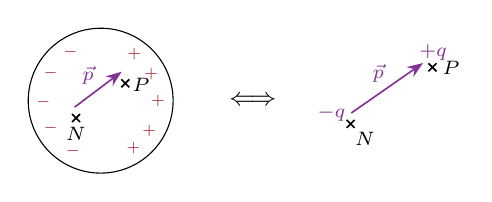
\begin{tikzpicture}[scale=.92]
 \draw(0,0)circle(1.0);
 \foreach \a in {54,28,0,-32,-55}{\node[rougechamp,font=\tiny,inner sep=0pt]at(\a:.79){$+$};}
 \foreach \a in {122,151,181,209,241}{\node[rougechamp,font=\tiny,inner sep=0pt]at(\a:.79){$-$};}
 \croix{-.34}{-.24}\croix{.34}{.24}
 \node[below,petit]at(-.34,-.31){$N$};\node[right,petit]at(.38,.22){$P$};
 \draw[moment](-.36,-.09)--(.29,.40)node[pos=.51,above left,petit]{$\mom$};
 \node at(2.10,0){$\Longleftrightarrow$};
 \croix{3.45}{-.32}\croix{4.58}{.46}
 \node[above left,petit,violetdip]at(3.44,-.34){$-q$};\node[below right,petit]at(3.45,-.37){$N$};
 \node[above,petit,violetdip]at(4.59,.50){$+q$};\node[right,petit]at(4.66,.45){$P$};
 \draw[moment](3.46,-.17)--(4.45,.52)node[pos=.52,above left,petit]{$\mom$};
\end{tikzpicture}}
\bmath{V(M)=\frac{\mom\cdot\fle{OM}}{4\pi\eps r^3}.}
\begin{exemple}\examtitle{Exemples}
L'eau \(\mathrm{H_2O}\), le chlorure d'hydrogène \(\mathrm{HCl}\) et l'ammoniac \(\mathrm{NH_3}\) sont des molécules polaires.
\end{exemple}
\titr{Troisième cas}
Si \(Q=0\) et \(\mom=\veczero\), il faut pousser plus loin le développement limité de \(1/P_iM\).

\begin{exemple}\examtitle{Molécule de \(\mathrm{CO_2}\)}
Cf. TD.
\fig{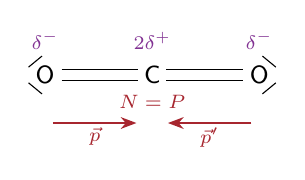
\begin{tikzpicture}
 \node[atome]at(-1.36,0){O};\node[atome]at(0,0){C};\node[atome]at(1.36,0){O};
 \draw(-1.15,.065)--(-.18,.065)(-1.15,-.065)--(-.18,-.065)
       (.18,.065)--(1.15,.065)(.18,-.065)--(1.15,-.065);
 \draw(-1.57,.10)--(-1.40,.24)(-1.57,-.10)--(-1.40,-.24)
      (1.40,.24)--(1.57,.10)(1.40,-.24)--(1.57,-.10);
 \node[violetdip,petit]at(-1.36,.44){$\delta^-$};\node[violetdip,petit]at(0,.43){$2\delta^+$};
 \node[violetdip,petit]at(1.36,.44){$\delta^-$};
 \node[rougechamp,petit]at(0,-.34){$N=P$};
 \draw[echamp](-1.26,-.61)--(-.20,-.61)node[midway,below,petit]{$\mom$};
 \draw[echamp](1.26,-.61)--(.20,-.61)node[midway,below,petit]{$\mom'$};
\end{tikzpicture}}
La distribution \(\D\) est neutre : \(Q=0\). Elle n'a pas de moment dipolaire :
\(\mom=\veczero\) car \(N=P\). Les deux moments de liaison se compensent : \(\mom+\mom'=\veczero\).
On obtient un terme \underline{quadripolaire}.
\end{exemple}
\titr{Conclusion}
Le potentiel créé en \(M\) par la distribution \(\D\) s'écrit
\[
 V(M)=\underbrace{\frac{Q}{4\pi\eps r}}_{\text{terme monopolaire}}
 +\underbrace{\frac{\mom\cdot\fle{OM}}{4\pi\eps r^3}}_{\text{terme dipolaire}}
 +\text{terme quadripolaire}+\cdots .
\]

% Manuscrit, pages 39 à 44.
\Needspace{57mm}
\subsection{Notion de polarisabilité}\label{sec:pol}
\titr{Dipôle induit}
Considérons l'atome d'hydrogène.
\fig{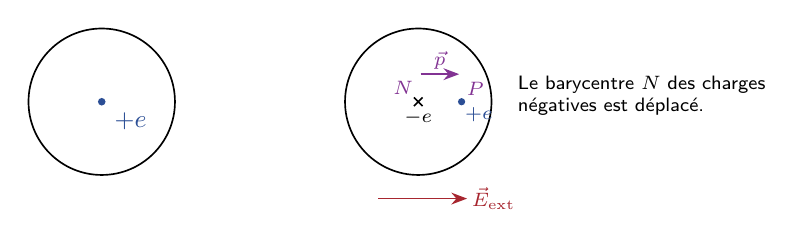
\begin{tikzpicture}
 \draw[semithick](0,0)circle(.93);\fill[bleutrait](0,0)circle(.048);
 \node[bleutrait,below right]at(.04,-.01){$+e$};
 \begin{scope}[shift={(4.02,0)}]
 \draw[semithick](0,0)circle(.93);
 \croix{0}{0}\node[violetdip,above left,petit]at(-.01,.04){$N$};\node[below,petit]at(0,-.05){$-e$};
 \fill[bleutrait](.55,0)circle(.046);
 \node[violetdip,above right,petit]at(.56,.02){$P$};\node[bleutrait,below right,petit]at(.54,-.02){$+e$};
 \draw[moment](.03,.35)--(.52,.35)node[midway,above,petit]{$\mom$};
 \draw[echamp](-.51,-1.23)--(.62,-1.23)node[right,petit]{$\EE$};
 \node[right,align=left,petit]at(1.21,.08){Le barycentre $N$ des charges\\ négatives est déplacé.};
 \end{scope}
\end{tikzpicture}}
\bmath{\mom=\alpha\eps\,\EE.}
Le coefficient \(\alpha\) est la \underline{polarisabilité}.

\titr{Dimension}
\[
 [\alpha]=\frac{[p]}{[\eps]\,[E]}=\frac{[q]\,L}{[q]\,L^{-2}}=L^3 .
\]
\titr{Ordre de grandeur}
La grandeur caractéristique est la taille de l'atome, de l'ordre de \(1~\text{\AA}\).
La polarisabilité est de l'ordre du volume de l'atome :
\(\alpha\simeq10^{-30}~\mathrm{m^3}\).

La valeur expérimentale pour l'atome d'hydrogène dans son état fondamental est
\[
 \alpha=8{,}4\times10^{-30}~\mathrm{m^3}.
\]
Pour obtenir un meilleur modèle, il faut faire appel à la mécanique quantique.

\titr{Énergie potentielle d'interaction}
\surdeux{.36}{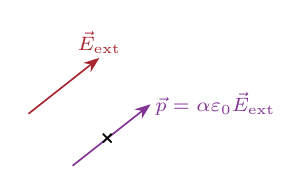
\begin{tikzpicture}
 \draw[echamp](-1.13,.03)--(-.23,.74)node[above,petit]{$\EE$};
 \draw[moment](-.57,-.63)--(.42,.15)node[right,petit]{$\mom=\alpha\eps\EE$};
 \croix{-.13}{-.28}
\end{tikzpicture}}{Les formules
\[
 \left\{\begin{aligned}
 \FR&=(\mom\cdot\grad)_O\,\EE,\\
 \MR&=\mom\wedge\EE(O)
 \end{aligned}\right.
\]
sont valables pour un dipôle rigide ou induit.}

Pour un dipôle induit, \(\mom=\alpha\eps\,\EE\). Ainsi, \(\MR=\veczero\) : le dipôle induit
ne subit pas de moment car il est toujours aligné avec \(\EE\), dans le même sens.
\begin{align*}
 \FR&=\big(\alpha\eps\,\EE\cdot\grad\big)_O\EE\\
 &=\alpha\eps\left[\frac12\grad \EEsc^2+
        \underbrace{\rot\EE}_{\veczero\ \text{en électrostatique}}\wedge\EE\right]\\
 &=\grad\left(\frac12\alpha\eps\EEsc^2\right)
 =-\grad E_p .
\end{align*}
L'énergie potentielle d'interaction d'un dipôle induit avec \(\EE\) vaut donc
\[
 E_{p,\mathrm{induit}}=-\frac12\eps\alpha\EEsc^2.
\]
\betoile{2}{E_{p,\mathrm{induit}}=-\frac12\,\mom\cdot\EE.}

\titr{Remarques}
\begin{itemize}
\item Un dipôle induit se déplace vers les zones de champ fort. En effet,
\(\FR=(\alpha\eps\,\EE\cdot\grad)_O\EE\) et le dipôle induit est toujours aligné avec \(\EE\).
Ce déplacement minimise l'énergie potentielle \(E_{p,\mathrm{induit}}=-\frac12\mom\cdot\EE\).
\end{itemize}
\begin{exemple}
\examtitle{Exemple}Une méthode industrielle permet de récupérer la poussière dans une cheminée.
\surdeux{.44}{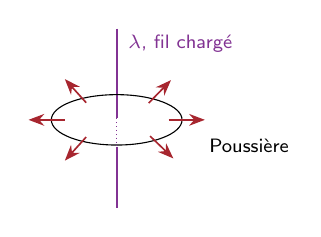
\begin{tikzpicture}
 \draw[violetdip,semithick](0,1.16)--(0,.02);
 \draw[thin](0,0)ellipse(.83 and .32);
 \draw[violetdip,densely dotted](0,.02)--(0,-.34);\draw[violetdip,semithick](0,-.34)--(0,-1.12);
 \foreach \a in {0,52,126,180,234,310}{
  \draw[echamp]({.66*cos(\a)},{.27*sin(\a)})--({1.12*cos(\a)},{.64*sin(\a)});}
 \node[violetdip,right,petit]at(.09,.97){$\lambda$, fil chargé};
 \node[right,petit]at(1.12,-.33){Poussière};
\end{tikzpicture}}{Un dipôle est induit sur chaque grain de poussière. Les grains se collent au fil.}
\end{exemple}
\begin{itemize}
\item La relation \(\vec F=-\grad(E_p)\) n'est valable que pour un point matériel.
On admet ici la validité du modèle.\label{err:gradient}
\item En toute rigueur, la formule \(E_{p,\mathrm{induit}}=-\tfrac12\mom\cdot\EE\)
n'est pas au programme.
\end{itemize}

% Manuscrit, pages 44 et 45.
\subsection{Approche descriptive de la solvatation}\label{sec:solv}
La solvatation a déjà été étudiée en chimie. Lorsqu'un cristal ionique est placé dans l'eau,
les ions se séparent sous l'effet des interactions entre les ions et les molécules d'eau.

Les ions sont des distributions monopolaires.
\fig{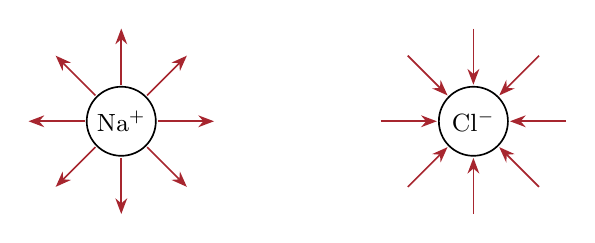
\begin{tikzpicture}[scale=.86]
 \foreach \x/\ion/\dir in {0/{\mathrm{Na}^+}/1,5.2/{\mathrm{Cl}^-}/-1}{\begin{scope}[shift={(\x,0)}]
  \draw[semithick](0,0)circle(.51);\node at(0,0){$\ion$};
  \foreach \a in {0,45,...,315}{
   \ifnum\dir=1 \draw[echamp](\a:.54)--(\a:1.37);
   \else \draw[echamp](\a:1.37)--(\a:.54);\fi}
 \end{scope}}
\end{tikzpicture}}

\surdeux{.31}{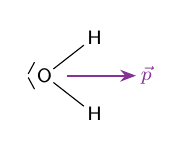
\begin{tikzpicture}[scale=1.14]
 \eau{(0,0)}{0}
 \draw[moment](.25,0)--(1.02,0)node[right,petit]{$\mom$};
\end{tikzpicture}}{La molécule d'eau est une distribution dipolaire.
Il s'agit donc d'une interaction charge-dipôle.}

\fig{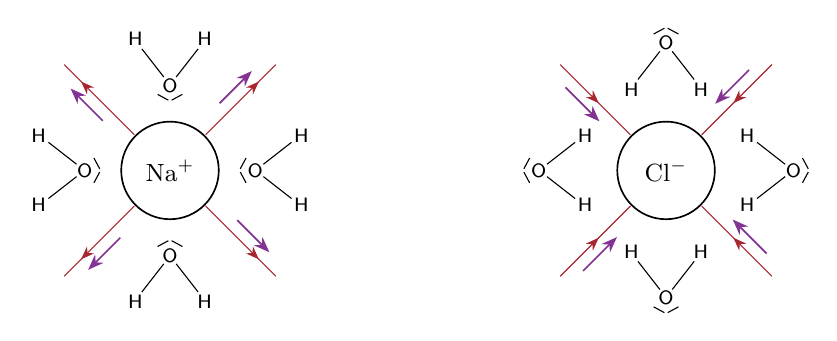
\begin{tikzpicture}[scale=1.05]
\foreach \decal/\ion/\dir in {0/{\mathrm{Na}^+}/1,6.0/{\mathrm{Cl}^-}/-1}{\begin{scope}[shift={(\decal,0)}]
 \draw[semithick](0,0)circle(.59);\node at(0,0){$\ion$};
 \foreach \a in {0,90,180,270}{
  \ifnum\dir=1 \pgfmathsetmacro{\distance}{1.03}\pgfmathsetmacro{\orient}{\a}
  \else \pgfmathsetmacro{\distance}{1.54}\pgfmathsetmacro{\orient}{\a+180}\fi
  \eau{({\distance*cos(\a)},{\distance*sin(\a)})}{\orient}}
 \foreach \a in {45,135,225,315}{\begin{scope}[rotate=\a]
  \ifnum\dir=1
   \draw[rougechamp,sens=.76](.61,0)--(1.81,0);
   \draw[moment](1.00,.15)--(1.55,.15);
  \else
   \draw[rougechamp,sens=.55](1.81,0)--(.61,0);
   \draw[moment](1.57,.15)--(.99,.15);
  \fi
 \end{scope}}
\end{scope}}
\end{tikzpicture}}

% Manuscrit, pages 45 à 47.
\subsection{Interaction de van der Waals}\label{sec:vdw}
À la fin du XIX\textsuperscript{e} siècle, pour une mole, on passe de la loi \(PV=RT\) à l'équation
\bmath{\left(P+\frac{a}{V^2}\right)(V-b)=nRT.}
\label{err:mole}
Pour \(n\) moles, on écrit
\[
 \left(P+\frac{n^2a}{V^2}\right)(V-nb)=nRT.
\]
Les deux termes correctifs, \(a/V^2\) et \(b\), traduisent les interactions entre molécules.

\surdeux{.53}{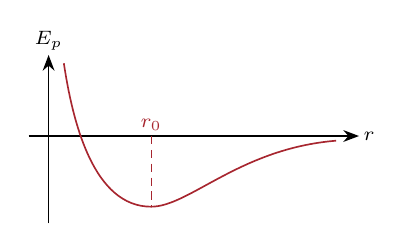
\begin{tikzpicture}[x=.88cm,y=.66cm]
 \draw[fl](-.29,0)--(4.48,0)node[right,petit]{$r$};
 \draw[fl](0,-1.68)--(0,1.56)node[above,petit]{$E_p$};
 \draw[rougechamp,semithick](.22,1.40)..controls(.35,.25)and(.65,-1.36)..(1.48,-1.36)
 ..controls(2.03,-1.36)and(2.76,-.24)..(4.15,-.09);
 \draw[rougechamp,densely dashed](1.48,0)--(1.48,-1.36);
 \node[rougechamp,above,petit]at(1.48,.03){$r_0$};
\end{tikzpicture}}{La distance \(r\) sépare les deux molécules.
\begin{itemize}
\item Pour \(r=r_0\), les molécules sont à l'équilibre.
\item Pour \(r>r_0\), la force est attractive.
\item Pour \(r<r_0\), la force est répulsive.
\end{itemize}}

\surdeux{.36}{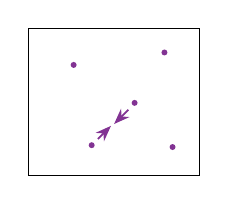
\begin{tikzpicture}[scale=.79]
 \draw(0,0)rectangle(2.76,2.37);
 \foreach \x/\y in {.73/1.78,2.19/1.98,1.71/1.17,1.02/.49,2.32/.46}{\fill[violetdip](\x,\y)circle(.048);}
 \draw[moment](1.61,1.06)--(1.38,.83);\draw[moment](1.12,.59)--(1.33,.80);
\end{tikzpicture}}{Le \textbf{covolume} \(b\) traduit l'interaction répulsive entre deux molécules :
chacune dispose de moins de volume accessible.}
\[
 P=\frac{RT}{V-b}-\frac{a}{V^2}.
\]
\surdeux{.36}{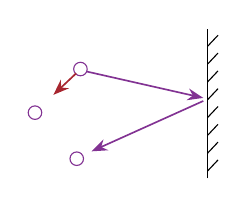
\begin{tikzpicture}[scale=.78]
 \draw[semithick](2.55,-.94)--(2.55,1.50);
 \foreach \y in {-.82,-.53,...,1.30}{\draw[thin](2.55,\y)--(2.72,{\y+.18});}
 \foreach \x/\y in {.48/.84,-.26/.13,.42/-.62}{\draw[violetdip](\x,\y)circle(.11);}
 \draw[moment](.58,.80)--(2.48,.37);\draw[moment](2.48,.32)--(.66,-.50);
 \draw[echamp](.41,.77)--(.04,.42);
\end{tikzpicture}}{Le terme correctif \(a/V^2\) traduit l'interaction attractive.}
\begin{cadre}L'interaction de van der Waals est une interaction attractive pour \(r>r_0\).\end{cadre}

% Manuscrit, pages 47 à 51.
\titr{Origine physique de cette interaction attractive}
% Une ligne de champ dans le plan du dipôle : r = k sin^2(theta).
\newcommand{\courbeDip}[3]{%
 \draw[rougechamp,thin]plot[domain=0:180,samples=70,smooth,variable=\t]
  ({#1*#2*sin(\t)^3},{#2*sin(\t)^2*cos(\t)});
 \foreach \tp in {#3}{\pgfmathsetmacro{\tb}{\tp-6}
  \draw[rougechamp,thin,-{Stealth[length=1.55mm,width=1.2mm]}]
   plot[domain=\tb:\tp,samples=5,smooth,variable=\t]
    ({#1*#2*sin(\t)^3},{#2*sin(\t)^2*cos(\t)});}}
\titr{1) Contribution de Keesom}
Elle correspond à l'interaction entre deux molécules polaires.
\fig{\begin{tikzpicture}[scale=.89]
 \begin{scope}
  \clip(-2.19,-1.48)rectangle(3.53,1.73);
  \begin{scope}[rotate=40]
   \courbeDip{-1}{1.28}{64,124}
   \courbeDip{1}{1.36}{53,122}
   \courbeDip{1}{5.7}{32,138}
  \end{scope}
 \end{scope}
 \croix{0}{0}\node[below left,petit]at(-.09,-.09){$O_1$};
 \draw[moment](.44,-.52)--(-.72,.86)node[above left,petit]{$\vec p_1$};
 \coordinate(OO) at ({5.7*sin(136)^2*cos(-6)},{5.7*sin(136)^2*sin(-6)});
 \draw[moment]($(OO)+(-.29,-.65)$)--($(OO)+(.42,.91)$)node[above right,petit]{$\vec p_2$};
 \draw[violetdip,thin,->]($(OO)+(.33,.48)$) to[bend right=20] ($(OO)+(.63,.15)$);
 \draw[violetdip,dashed,fl]($(OO)+(-.14,.02)$)--($(OO)+(-.97,.06)$);
 \fill(OO)circle(.046);\node[below right,petit]at($(OO)+(.03,-.04)$){$O_2$};
\end{tikzpicture}}
Le dipôle de moment \(\vec p_2\) s'aligne sur le champ créé par \(\vec p_1\), puis
se rapproche de la zone de champ fort. Il en va de même pour l'action de \(\vec p_2\) sur \(\vec p_1\), selon le principe des actions réciproques.

Le champ dipolaire vérifie \(E_{\text{dipôle}}\propto1/r^3\).
La loi \(F_{1\to2}\propto1/r^3\) est écartée.\label{err:keesom}
L'alignement fluctue sous l'effet de l'agitation thermique. La physique statistique donne
\[
 F\sim\frac{1}{r^7},\qquad E_p\sim\frac{1}{r^6}.
\]
Toutefois,
\[
 \left(\frac{a}{r^2}\right)_{\text{calculé}}<
 \left(\frac{a}{r^2}\right)_{\text{expérimental}}.
\]\label{err:pression}

\titr{2) Contribution de Debye}
Elle correspond à l'interaction entre une molécule polaire et une molécule polarisable.
\surdeux{.45}{\begin{tikzpicture}[scale=.78]
 \begin{scope}[rotate=-32]
  \courbeDip{-1}{1.02}{75,129}
  \courbeDip{1}{1.03}{64,121}
  \courbeDip{1}{3.02}{51,129}
 \end{scope}
 \croix{0}{0}\node[below left,petit]at(-.20,-.08){$O_1$};
 \draw[moment](-.55,-.88)--(.72,1.15)node[above,petit]{$\vec p_1$};
 \coordinate(OO) at ({3.02*sin(86)^2*cos(-28)},{3.02*sin(86)^2*sin(-28)});
 \fill(OO)circle(.046);\node[right,petit]at($(OO)+(.08,0)$){$O_2$};
 \draw[moment]($(OO)+(.10,.24)$)--($(OO)+(-.29,-.72)$)
  node[below right,petit]{$\vec p_2$ induit};
\end{tikzpicture}}{L'interaction est attractive. Avec la physique statistique, on retrouve les dépendances
\[
 F\propto\frac1{r^7},\qquad E_p\propto\frac1{r^6}.
\]}
On a toujours
\[
 \left(\frac{a}{r^2}\right)_{\text{calculé}}<
 \left(\frac{a}{r^2}\right)_{\text{expérimental}}.
\]

\Needspace{75mm}
\titr{3) Contribution de London}
Elle intervient entre deux molécules non polaires.
\surdeux{.33}{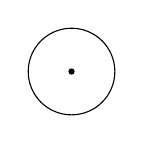
\begin{tikzpicture}
 \draw(0,0)circle(.55);\fill(0,0)circle(.04);
\end{tikzpicture}}{En moyenne, \(\mom=\veczero\) et les barycentres \(N\) et \(P\) coïncident.}
À un instant donné, \(\mom(t)\ne\veczero\).
\surdeux{.33}{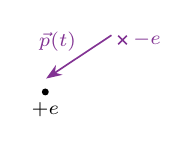
\begin{tikzpicture}
 \croix[violetdip]{.66}{.35}\node[violetdip,right,petit]at(.74,.35){$-e$};
 \fill(-.32,-.31)circle(.044);\node[below,petit]at(-.32,-.39){$+e$};
 \draw[moment](.52,.41)--(-.31,-.14)node[pos=.47,above left,petit]{$\mom(t)$};
\end{tikzpicture}}{L'interprétation fait intervenir la mécanique quantique et la physique statistique.}
L'interaction est attractive :
\[
 F\sim\frac1{r^7},\qquad E_p\sim\frac1{r^6}.
\]
En sommant les trois interactions, on obtient
\[
 \left(\frac a{r^2}\right)_{\text{\scriptsize\zone{1}}}+
 \left(\frac a{r^2}\right)_{\text{\scriptsize\zone{2}}}+
 \left(\frac a{r^2}\right)_{\text{\scriptsize\zone{3}}}
 =\left(\frac a{r^2}\right)_{\text{expérimental}}.
\]

\titr{Remarques}
\begin{itemize}
\item En thermodynamique, ces interactions interviennent dans les températures de changement d'état.
\item Elles ont également des conséquences en cristallographie.
\item En catalyse hétérogène, il existe des interactions de van der Waals entre un gaz et une paroi.
\item La tension superficielle intervient dans les phénomènes d'interface à la surface d'un fluide.
\begin{exemple}\textbf{Exemple}\par Un ménisque se forme dans un tube à essai.\end{exemple}
\end{itemize}
\end{document}